\chapter{Marco teórico }

\hrule \bigskip \vspace*{1cm}

%El Marco Teórico es el conjunto de conceptos y bases teóricas necesarias para la comprensión y entendimiento de los diferentes componentes, pasos o etapas planteados en la propuesta del trabajo. Esto permitirá comprender los diferentes conceptos y términos utilizados en todo el trabajo de investigación.
\subsection{SRC y SCL}


La medición de la actividad electrodermica (EDA)  se compone de  dos partes: 

 
\begin{itemize}
    \item \textbf{El nivel de conductancia tónico de la piel(SCL):}Se muestra en la imagen \ref{fig:src}como la señal suave subyacentes que cambia lentamente.
    Se da en ausencia de cualquier evento ambiental discreto particular o estímulos externos. El nivel de conductancia tónica de la piel puede variar lentamente con el tiempo en un individuo dependiendo de su estado psicológico, hidratación, sequedad de la piel.
    \item \textbf{Respuesta  de la Conductancia Cutánea(SRC):}
     Son aumentos bruscos de la conductancia de la piel ,  los picos  en  la Figura \ref{fig:src2}.Se asocian típicamente con eventos a corto plazo y ocurren en presencia de estímulos ambientales discretos: vista, sonido, olfato, procesos cognitivos que preceden a un evento, como anticipación, toma de decisiones, etc. 
\end{itemize}

\begin{figure}[h]
    \centering
    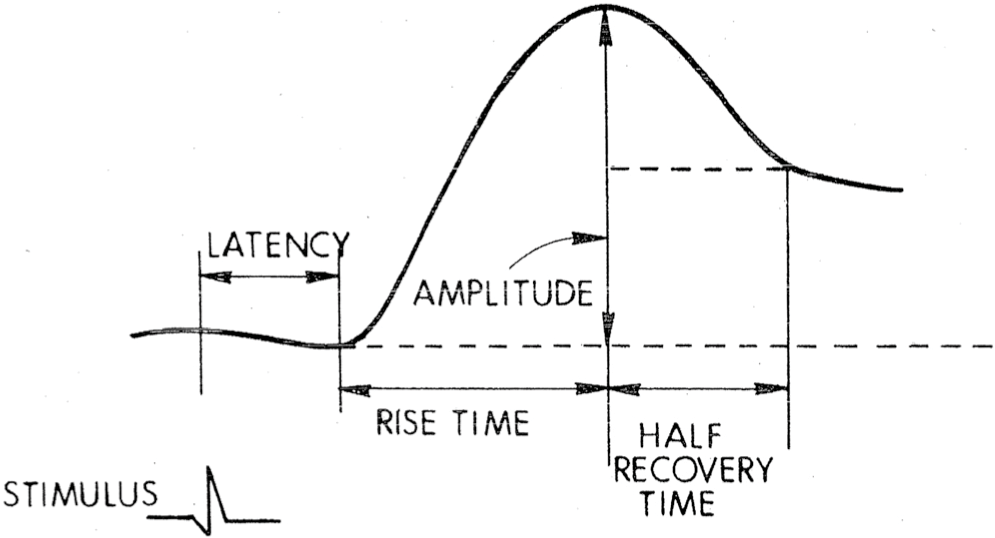
\includegraphics[width=10cm]{Graficos/senal.png}
    \caption{ Visualización de los componentes de un SRC ante un evento .Dawson et al.[Dawson et al,2017] }
    \label{fig:src2}
\end{figure}

\begin{figure}[h]
    \centering
    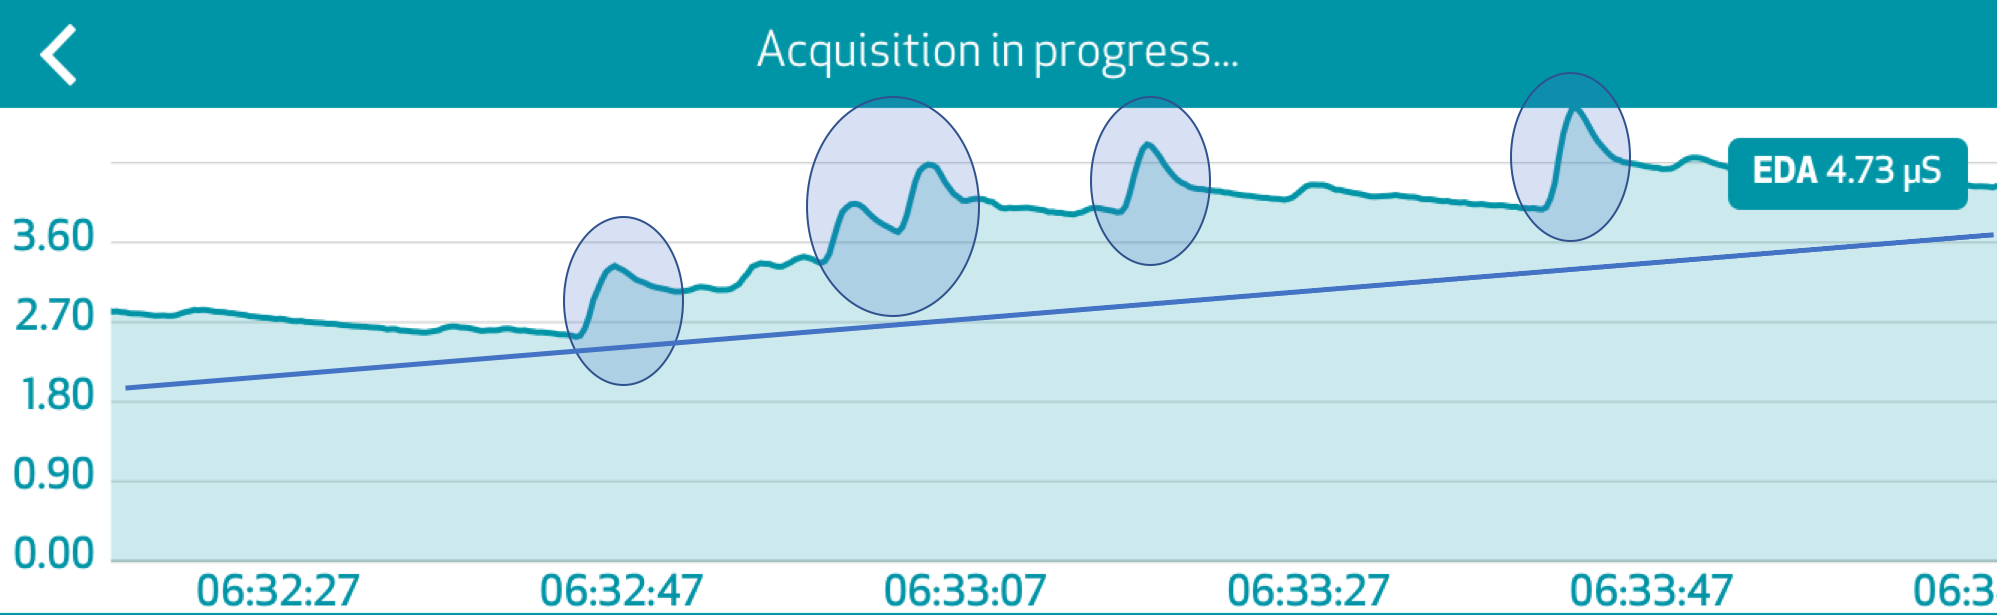
\includegraphics[width=15cm]{Graficos/new_EDA_figure.png}
    \caption{ Señal EDA capturado de la Aplicación Empatica Realtime}
    \label{fig:src}
\end{figure}

\begin{figure}[h]
    \centering
    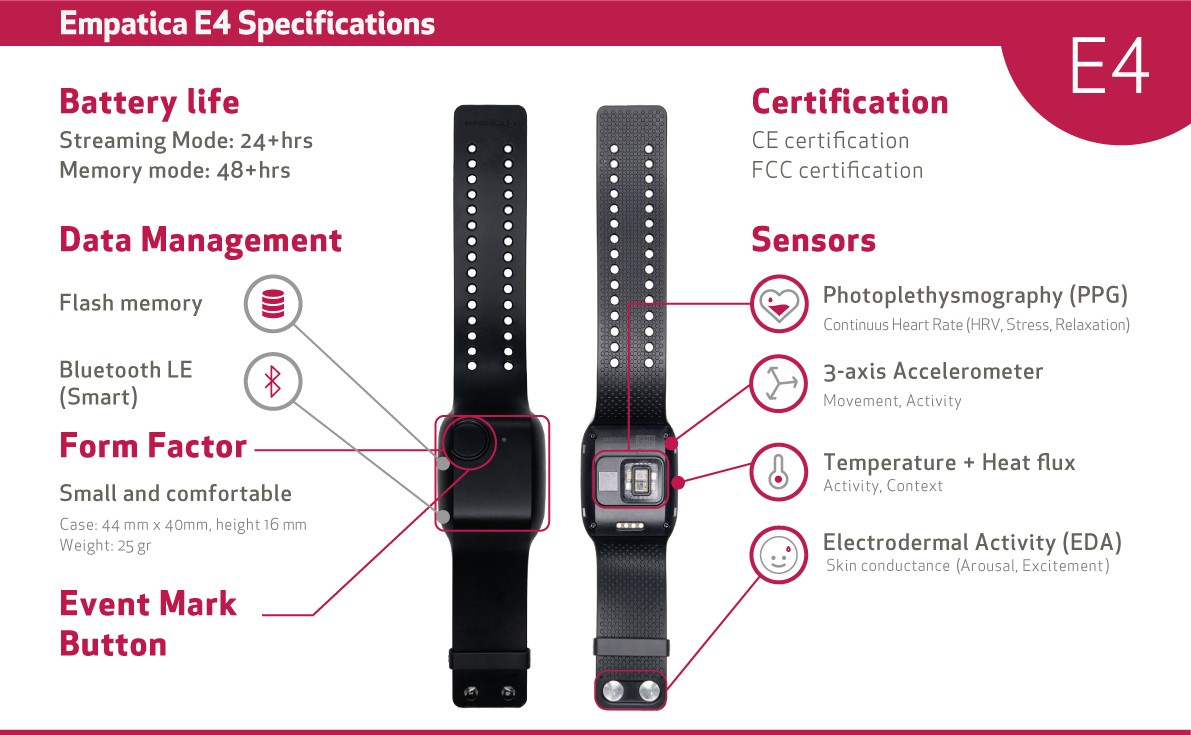
\includegraphics[width=15cm]{Graficos/e4specs.jpg}
    \caption{ Especificaciones técnicas del E4-wristband}
    \label{fig:relo}
\end{figure}

    
    
    